\subsection{真实地图上：躲比跑活得久，优势主要来自藏身处本身}
\label{sec:res-campus}
图~\ref{fig:campus}a 是基准条件下五种策略的存活曲线，表~\ref{tab:campus} 给出各条件下的平均存活和以跑为对照的局内配对差。基准条件下，就近选灌木或夹缝的“躲”平均活 11.2 分钟，比跑多 5.8 分钟（95\% 区间 [4.9, 6.7]）；只躲夹缝与它几乎一样，11.1 分钟；原地不动 8.5 分钟，只躲灌木 6.3 分钟，也都好过跑（5.4 分钟）。“躲”和“只躲夹缝”分别有 28\% 和 27\% 的老鼠撑满了 30 分钟，跑的老鼠只有 3\%。所以 RQ1 的第一问得到了肯定的回答：在这片校园里，躲确实比跑活得久。

\begin{figure}[htbp]
  \centering
  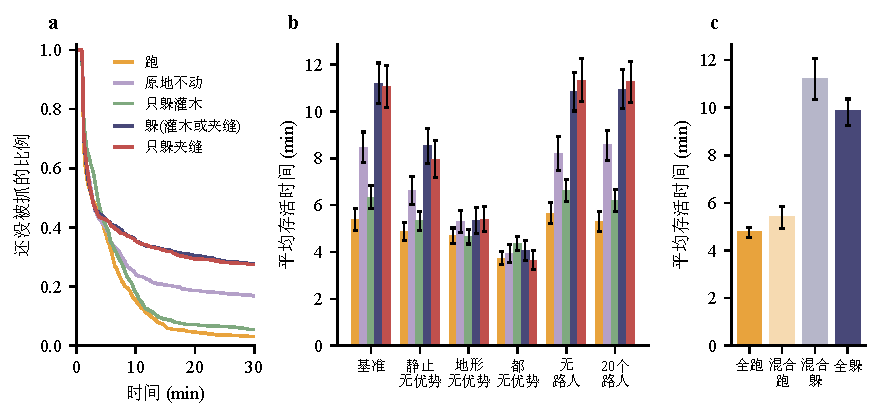
\includegraphics[width=\textwidth]{fig3_campus_hide_vs_run.pdf}
  \caption{\figlead{在真实地图上躲比跑活得久；取消藏身处的隐蔽优势后，躲的优势大部分消失。}
  \textbf{a}，基准条件下五种策略的存活曲线（每种策略 1024 只老鼠，一轮 30 分钟）。
  \textbf{b}，六种条件下的平均存活时间：基准；静止无优势（$f_{\text{静}}=1$）；地形无优势（$f_{\text{灌木}}=f_{\text{夹缝}}=1$）；两者都无优势；无夜跑路人；20 个路人。颜色同 \textbf{a}，误差棒为按局自举的 95\% 区间，每种条件 256 局。
  \textbf{c}，全跑、全躲两种同质群体与混合群体的对比（每组 256 局）。浅色柱是混合群体中该策略老鼠的人均存活。}
  \label{fig:campus}
\end{figure}

\begin{table}[htbp]
  \centering\small
  \caption{真实地图上各策略的平均存活（分钟）与“该策略 − 跑”的局内配对差。方括号是按局自举的 95\% 区间，每格 256 局 × 4 只老鼠。}
  \label{tab:campus}
  \footnotesize\setlength{\tabcolsep}{2.5pt}
  \begin{tabular}{@{}lccccc@{}}
    \toprule
    条件 & 跑 & 原地不动 & 只躲灌木 & 躲（灌木或夹缝） & 只躲夹缝\\
    \midrule
    % 以下各行由 catmouse/make_tables.py 生成
    基准 & 5.4 & 8.5（+3.1 [2.3, 3.9]） & 6.3（+1.0 [0.3, 1.7]） & 11.2（+5.8 [4.9, 6.7]） & 11.1（+5.7 [4.8, 6.6]）\\
    静止无优势 & 4.9 & 6.6（+1.7 [1.1, 2.4]） & 5.3（+0.4 [$-$0.1, 1.0]） & 8.5（+3.7 [2.8, 4.5]） & 7.9（+3.0 [2.3, 3.9]）\\
    地形无优势 & 4.7 & 5.3（+0.6 [0.0, 1.2]） & 4.6（$-$0.0 [$-$0.5, 0.4]） & 5.3（+0.6 [0.0, 1.2]） & 5.4（+0.7 [0.1, 1.3]）\\
    两者都无优势 & 3.7 & 3.9（+0.2 [$-$0.3, 0.6]） & 4.3（+0.6 [0.2, 1.0]） & 4.1（+0.3 [$-$0.2, 0.8]） & 3.6（$-$0.1 [$-$0.6, 0.4]）\\
    无夜跑路人 & 5.7 & 8.2（+2.6 [1.8, 3.3]） & 6.6（+1.0 [0.4, 1.6]） & 10.8（+5.2 [4.3, 6.1]） & 11.3（+5.7 [4.7, 6.7]）\\
    20 个路人 & 5.3 & 8.6（+3.3 [2.5, 4.0]） & 6.2（+0.9 [0.3, 1.5]） & 10.9（+5.6 [4.8, 6.5]） & 11.3（+6.0 [5.1, 6.9]）\\
    \bottomrule
  \end{tabular}
\end{table}

第二问是：躲的优势靠的是什么？这里要用到第~\ref{sec:detect} 节的反事实对照。现实中藏在夹缝里、站着不动当然更难被发现，把系数改成 1 并不是说现实不是这样，而是看“如果没有这一条，躲还剩多少优势”。结果如下：

\begin{itemize}
  \item \textbf{只取消地形的隐蔽优势}（灌木、夹缝和平地一样显眼）：躲的优势从 +5.8 分钟降到 +0.6 分钟，夹缝从 +5.7 降到 +0.7 分钟，和“原地不动”剩下的优势（+0.6 分钟）一样。也就是说，藏身处一旦不再更隐蔽，躲进去就和在空地上站着不动没有区别。
  \item \textbf{只取消静止的隐蔽优势}（站着和走动一样显眼）：躲仍然比跑多活 3.7 分钟，夹缝多活 3.0 分钟。躲的优势少了约三分之一，所以“站着不动”有贡献，但不是主要原因。
  \item \textbf{两者都取消}（怎么藏、动不动都一样显眼）：跑只剩 3.7 分钟，躲比跑多 0.3 分钟（[$-$0.2, 0.8]），夹缝少 0.1 分钟（[$-$0.6, 0.4]），原地不动多 0.2 分钟（[$-$0.3, 0.6]）。躲的优势完全消失，区间都包含 0。
\end{itemize}

因此，躲赢在“藏身处本身难被看见”，再加上“藏好后不动”锦上添花；单靠在空地上站着不动只能多活 3 分钟左右。这回答了 RQ1 的第二问。夜跑路人的影响很小：路人从 0 增加到 20 个，跑的老鼠只少活 0.4 分钟（5.7 → 5.3），躲的老鼠几乎不变（10.8 → 10.9），区间互相重叠。认错路人的代价不大：老鼠冲刺跑开，路人不会追，体力很快又恢复了。

图~\ref{fig:campus}c 比较了同质群体和混合群体。全跑群体人均 4.8 分钟（[4.6, 5.0]），混在其他策略中间的跑者 5.4 分钟；全躲群体人均 9.8 分钟，混合群体中的躲者 11.2 分钟。被抓即转化意味着每个被抓的人都会给别人多添一只猫，所以别人的策略在原理上会影响自己的存活；但从数值看，这种影响只有 0.6–1.4 分钟，远小于自己选躲还是选跑带来的 5–6 分钟的差别。第~\ref{sec:res-rounds} 节的收益曲线给出同样的结论。
